\section{Tangential Acceleration and Centripetal Acceleration}

\begin{comment}
This lab is new in fall 2019 by Matt Trawick.  I ran this for the very first time in my class this fall, and it seemed
to work fine.  The students also said it went okay.  

This lab is meant to address a topic my students have generally found confusing.  I

\end{comment}

\makelabheader %(Space for student name, etc., defined in master.tex or labmanual_formatting_commands.tex)

\textbf{Activity}

1. The picture below shows a top view of a car speeding up while taking a curve on a road. 

(a)  Use graphical techniques (no calculations) to draw a vector representing the change in velocity $\Delta \vv{v}$ during the time shown.

\hspace{1.0in}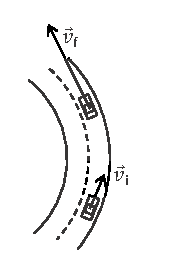
\includegraphics{tangential_and_centripetal_acc/curve1.eps}

(b) Does the average acceleration $\vv{a}_{\rm avg}$ during this time point towards the center of the curve?
\answerspace{0.3in}


(c) You may have done previous exercises
that involved a car driving on a circular track, in which the average acceleration always pointed towards the center of the curve.  
\iflabelexists{vector_addition_exercises}{(See Lab \ref{vector_addition_exercises}, for instance.)}{}
Why is the case pictured above different?
\answerspace{0.3in}

2.  (a) Suppose you are driving north on a straight road.  You accelerate uniformly from rest to a speed of 15~m/s over a time $\Delta t = 5$ seconds.  What is the magnitude and direction of your accleration $\vv{a}$ during this time?  Also draw your acceleration vector $\vv{a}$ on the picture below.

\hspace{1.0in}
\includegraphics{tangential_and_centripetal_acc/straight.eps}

(b) Now suppose you are driving at a constant speed $v=10$~m/s around a curve of radius $R=25$~m.  What is the magnitude and direction of your acceleration $\vv{a}$ at exactly the moment pictured below?  Also draw your acceleration vector $\vec{a}$ on the picture.

\hspace{1.0in}
\includegraphics{tangential_and_centripetal_acc/curve2.eps}

\pagebreak[3]
(c) Finally, suppose that you 
%combine the change in your speed from part (a) with the turn in part (b).  That is, you 
accelerate from 0~m/s to 15~m/s over $\Delta t = 5$ seconds like you did in part (a), but you do it while taking the same curve in the road as in part (b).  That is, you use the gas pedal to give your car an acceleration as you did in part (a), while also using the steering wheel to give your car an acceleration like you did in part (b). At the moment shown in the picture below, you happen to have a speed of exactly $v=10$~m/s.  Draw your acceleration vector $\vv{a}$ on the picture below.

\hspace{1.0in}
\includegraphics{tangential_and_centripetal_acc/curve2.eps}

(d) What is the centripetal component of your acceleration $a_c$?  (That is, the component of your acceleration vector towards the center or the curve.)
\answerspace{0.3in}

(e) What is the tangential component of your acceleration $a_t$?  (That is, the component of your acceleration vector along your direction of motion.)
\answerspace{0.3in}

(f) What is the magnitude and direction of your acceleration $\vv{a}\,$?
\answerspace{1.5in}

(g) In what direction is the net force $\vv{F}_{\rm NET}$ on your car at this time?
\answerspace{0.5in}



